\documentclass[12pt, a4paper, oneside]{ctexart}
\usepackage{amsmath, amsthm, amssymb, appendix, bm, graphicx, hyperref, mathrsfs}
\usepackage{algorithm,algorithmic}
\usepackage{caption}
\usepackage{listings}
\lstset{
	basicstyle=\ttfamily,
	frame=single
}
\renewcommand{\lstlistingname}{列表}
\title{\textbf{论文标题}}
\author{Dylaaan}
\date{\today}
\linespread{1.5}

\newtheorem{theorem}{定理}[section]
\newtheorem{definition}[theorem]{定义}
\newtheorem{lemma}[theorem]{引理}
\newtheorem{corollary}[theorem]{推论}
\newtheorem{example}[theorem]{例}
\newtheorem{proposition}[theorem]{命题}
\renewcommand{\abstractname}{\Large\textbf{摘要}}

\begin{document}
\maketitle

\setcounter{page}{0}
\maketitle
\thispagestyle{empty}

\begin{lstlisting}[caption={Shared element},label=l1]
class sharedElem(sdata, idx):
	cluId = idx
	isMark = 0
	data = sdata
	isCore = 0
	resCId = 0
\end{lstlisting}

\begin{algorithm}[htbp]
	\renewcommand{\algorithmicrequire}{\textbf{输入:}}
	\renewcommand{\algorithmicensure}{\textbf{输出:}}
	\caption{SMin(S) $\rightarrow \{\langle r_1 \rangle,...,\langle r_n\rangle\}$}
	\label{alg_sc}
	\begin{algorithmic}[1]
		\REQUIRE $C_0,C_1$输入$ \{\langle x_1 \rangle,...,\rangle x_n\rangle\} $
		\ENSURE $C_0,C_1$获得$\{\langle r_1 \rangle,...,\langle r_n\rangle\}$
		\STATE 构造$ n(n-1) $对比较数据,分别存储在$ l_1 $和$ l_2 $中
		\FOR{$i=1$ to $n$}
		\FOR{$j=1$ to $ n $, $j\neq i$}
		\STATE $ l_1[i*(n-1)+j] \leftarrow \langle x_i \rangle $
		\STATE $ l_2[i*(n-1)+j] \leftarrow \langle x+j \rangle $
		\ENDFOR
		\ENDFOR
		\STATE 比较大小获取结果$ \langle t \rangle \leftarrow \text{SC}(l_1, l_2) $
		\FOR{$ i=1 $ to $n$}
		\STATE 将$ \langle x_i\rangle $相关比较结果相乘$ \langle r_i \rangle \leftarrow \text{MUL}(\langle t_{i*(n-1)+1}\rangle,...,\langle t_{i*n} \rangle)$
		\ENDFOR
	\end{algorithmic}
\end{algorithm}

\begin{algorithm}[htbp]
	\renewcommand{\algorithmicrequire}{\textbf{输入:}}
	\renewcommand{\algorithmicensure}{\textbf{输出:}}
	\caption{SMin(L) $\rightarrow \{\langle r_1  \rangle,...,\langle r_n\rangle\}$}
	\label{alg_sminl}
	\begin{algorithmic}[1]
		\REQUIRE $C_0,C_1$输入$ \{\langle x_1 \rangle,...,\rangle x_n\rangle\} $
		\ENSURE $C_0,C_1$获得$\{\langle r_1 \rangle,...,\langle r_n\rangle\}$
		\FOR{$ i=1 $ to $ n/2 $}
		\STATE 
		\ENDFOR
		\STATE 构造$ n(n-1) $对比较数据,分别存储在$ l_1 $和$ l_2 $中
		\FOR{$i=1$ to $n$}
		\FOR{$j=1$ to $ n $, $j\neq i$}
		\STATE $ l_1[i*(n-1)+j] \leftarrow \langle x_i \rangle $
		\STATE $ l_2[i*(n-1)+j] \leftarrow \langle x+j \rangle $
		\ENDFOR
		\ENDFOR
		\STATE 比较大小获取结果$ \langle t \rangle \leftarrow \text{SC}(l_1, l_2) $
		\FOR{$ i=1 $ to $n$}
		\STATE 将$ \langle x_i\rangle $相关比较结果相乘$ \langle r_i \rangle \leftarrow \text{MUL}(\langle t_{i*(n-1)+1}\rangle,...,\langle t_{i*n} \rangle)$
		\ENDFOR
	\end{algorithmic}
\end{algorithm}


\newpage

本文算法的核心思想是,令核心对象与其$ \epsilon $范围内未被划分的边界对象组成独立的临时簇,临时簇内所有数据对象的簇标识保持一致。
在遍历的过程中对于核心对象,修改其$ \epsilon $范围内未被划分的边界对象的簇标识,与当前核心对象保持一致。对于核心对象$ \epsilon $范围内的其他核心对象,记录二者的相邻关系。
在还原聚类结果时,根据相邻关系构造邻接矩阵(相邻对象对应值大于0),通过深度优先遍历算法找到相邻的临时簇合并,不相邻的临时簇不受影响。

假设当前有一个包含10个点的数据集$ \{p_1,...,p_{10}\} $,令minPts为2,用圆圈框出所有数据对象的$ \epsilon $邻域,数据集可视化后如\ref{dataraw}所示,其中虚线框为边界对象$ \epsilon $邻域,实线框为核心对象$ \epsilon $邻域。
在图\ref{dbraw}中,我们用蓝色表示核心对象,绿色表示边界对象,噪声点在聚类过程中不会进行任何处理,为了简化表示,示例数据集没有噪声点。
\begin{figure}[htbp]
	%	\centering
	\begin{minipage}[t]{0.48\linewidth}
		\centering
		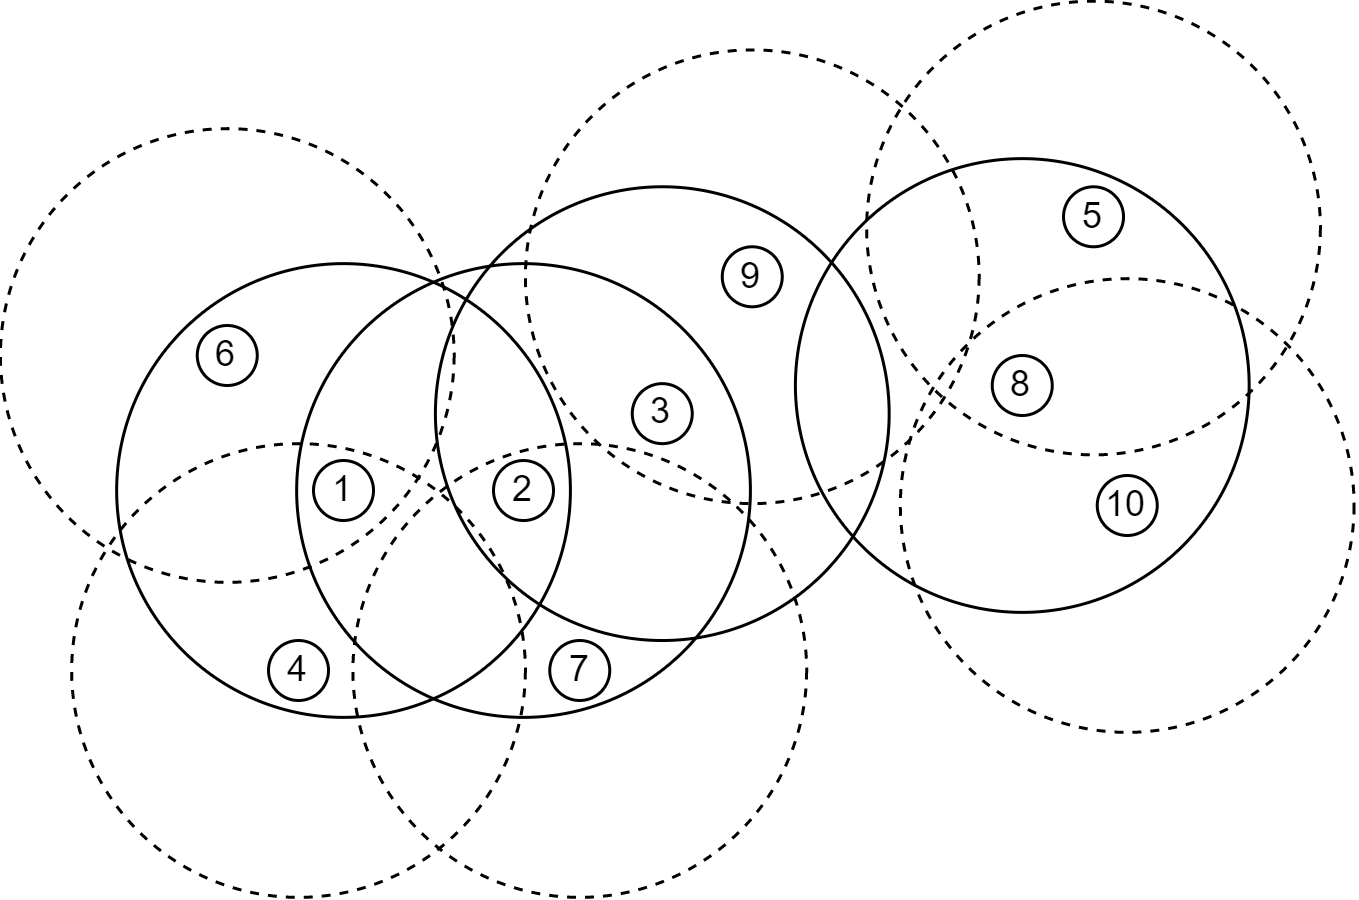
\includegraphics[width=\linewidth]{../img/dbraw.png}
		\caption{数据可视化}
		\label{dataraw}
	\end{minipage}
	\hfill
	\begin{minipage}[t]{0.48\linewidth}
		\centering
		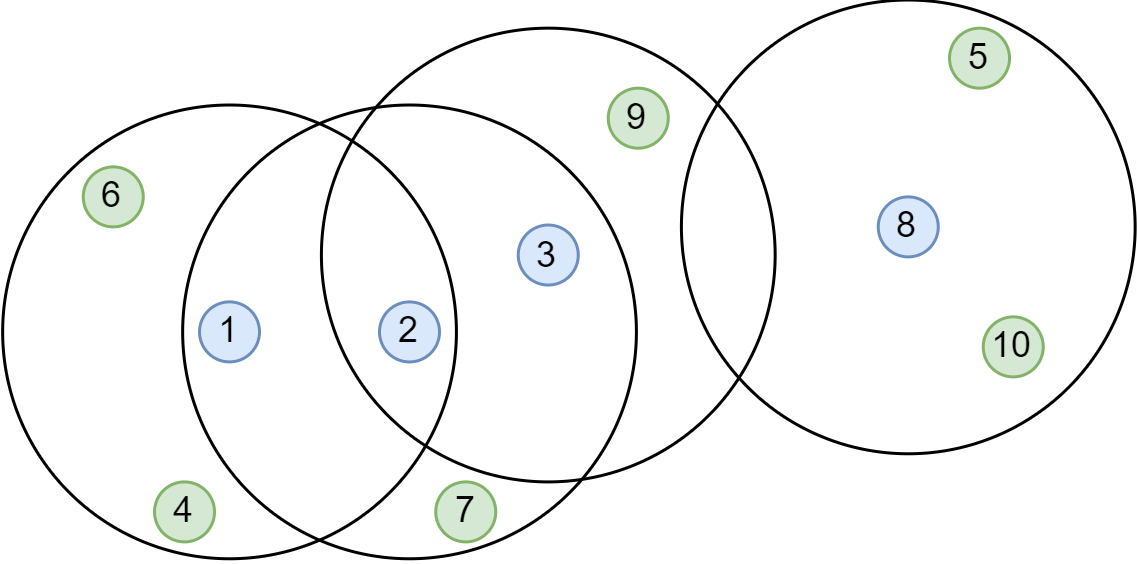
\includegraphics[width=\linewidth]{../img/db1.png}
		\caption{核心对象与边界对象}
		\label{dbraw}
	\end{minipage}
\end{figure}

接下来,在上述示例数据集的基础上,将详细介绍聚类的过程。按照编号$ \{1,2,...,10\} $进行遍历,每一个数据对象的初始簇标识为图中序号。首先,对$ p_1 $进行处理,在其$ \epsilon $范围内,有边界对象$ p_6$,$p_4 $和核心对象$ p_2 $。针对边界对象,我们修改其编号与$ p_1 $保持一致;针对核心对象,我们记录相邻关系;不在$ \epsilon $范围内的点(例如$ p_3 $和$ p_9 $),不做任何处理。遍历完结果如图\ref{db1}所示,这里对处理过的内容进行颜色加深。其他核心对象($ p_2 $,$ p_3 $,$ p_8 $)的处理和$ p_1 $一致,最后遍历完成的结果如图\ref{db4}所示。

\begin{figure}[htbp]
	\begin{minipage}[t]{0.24\linewidth}
		\centering
		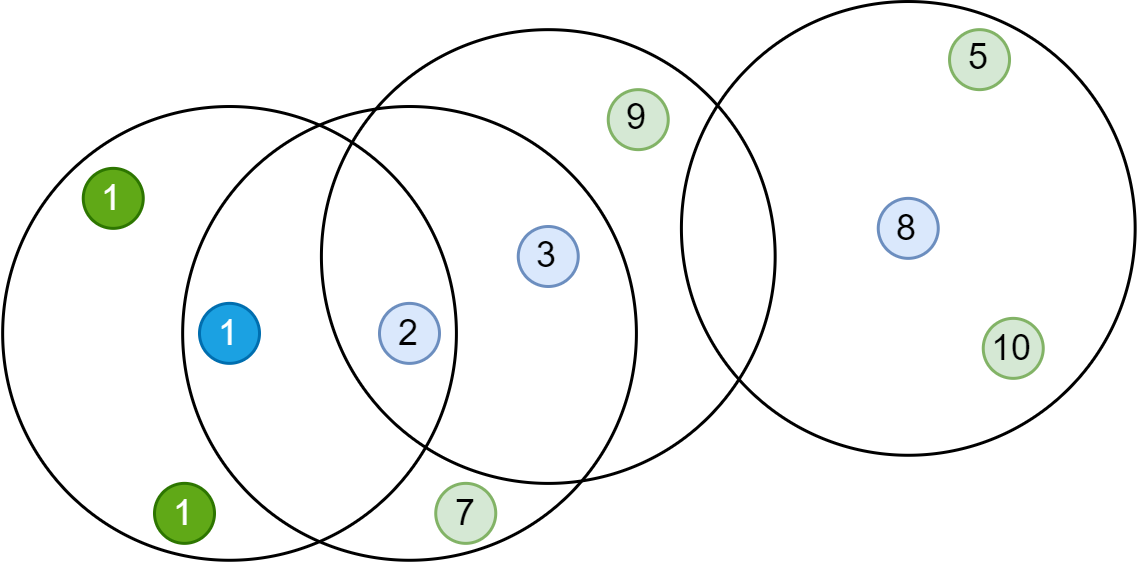
\includegraphics[width=\linewidth]{../img/db2.png}
		\caption{处理$ p_2 $}
		\label{db2}
	\end{minipage}
\hfill
	\begin{minipage}[t]{0.24\linewidth}
		\centering
		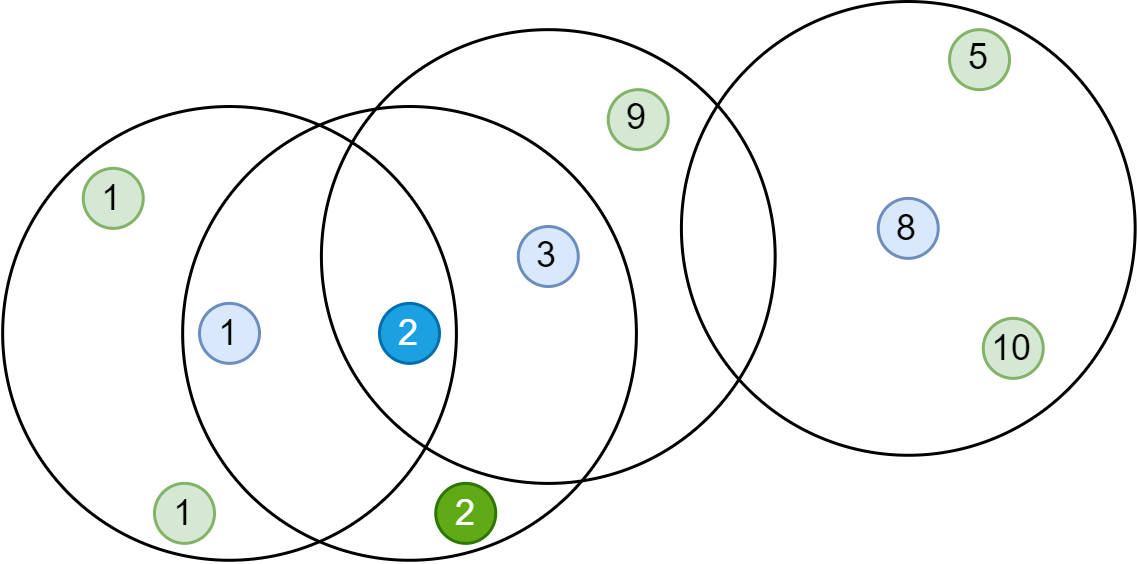
\includegraphics[width=\linewidth]{../img/db3.png}
		\caption{处理$ p_2 $}
		\label{db2}
	\end{minipage}
\hfill
	\begin{minipage}[t]{0.24\linewidth}
	\centering
	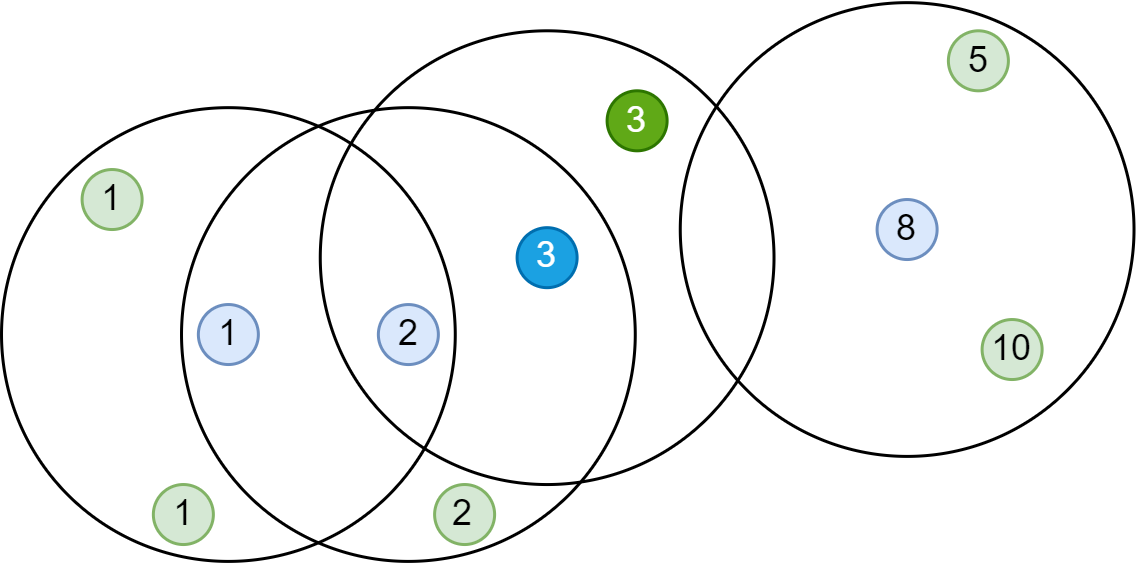
\includegraphics[width=\linewidth]{../img/db4.png}
	\caption{处理$ p_3 $}
	\label{db3}
	\end{minipage}
\hfill
	\begin{minipage}[t]{0.24\linewidth}
	\centering
	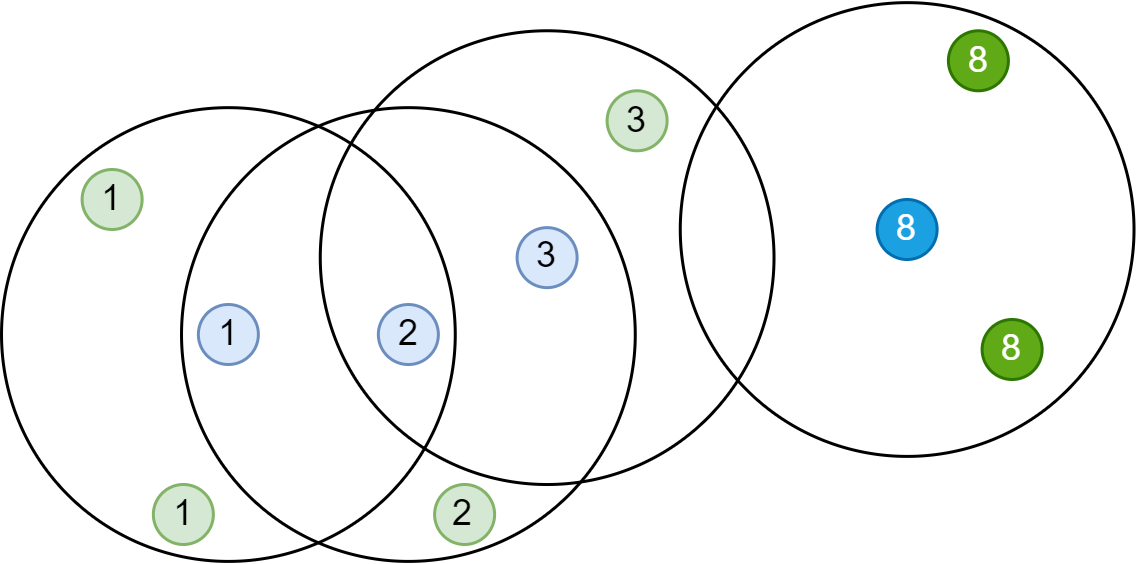
\includegraphics[width=\linewidth]{../img/db5.png}
	\caption{处理$ p_8 $}
	\label{db4}
	\end{minipage}
\end{figure}

接下来,我们根据遍历过程中存储的相邻关系构造矩阵,结果如图\ref{db_matrix}所示,可以看到只有核心点之间的存在相连关系(灰色部分)。基于该邻接矩阵,运行深度优先遍历算法,可以将临时簇进行合并。

\begin{figure}[htbp]
	\centering
	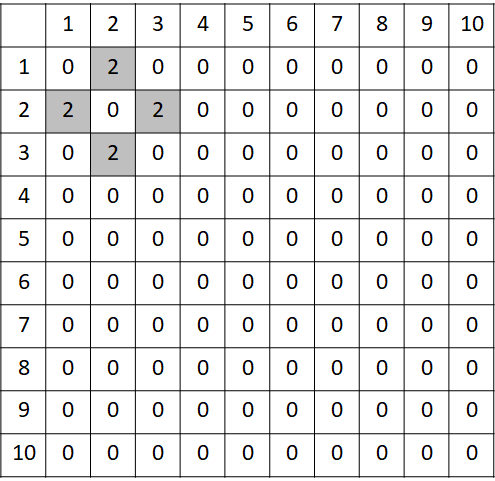
\includegraphics[width=0.4\textwidth]{../img/db_matrix.png}
	\caption{相连关系}
	\label{db_matrix}
\end{figure}

经过合并后,得到最终聚类结果,数据集包含两个簇,如图\ref{dbres}所示,其中黄色为簇1,紫色为簇2。

\begin{figure}[htbp]
	\centering
	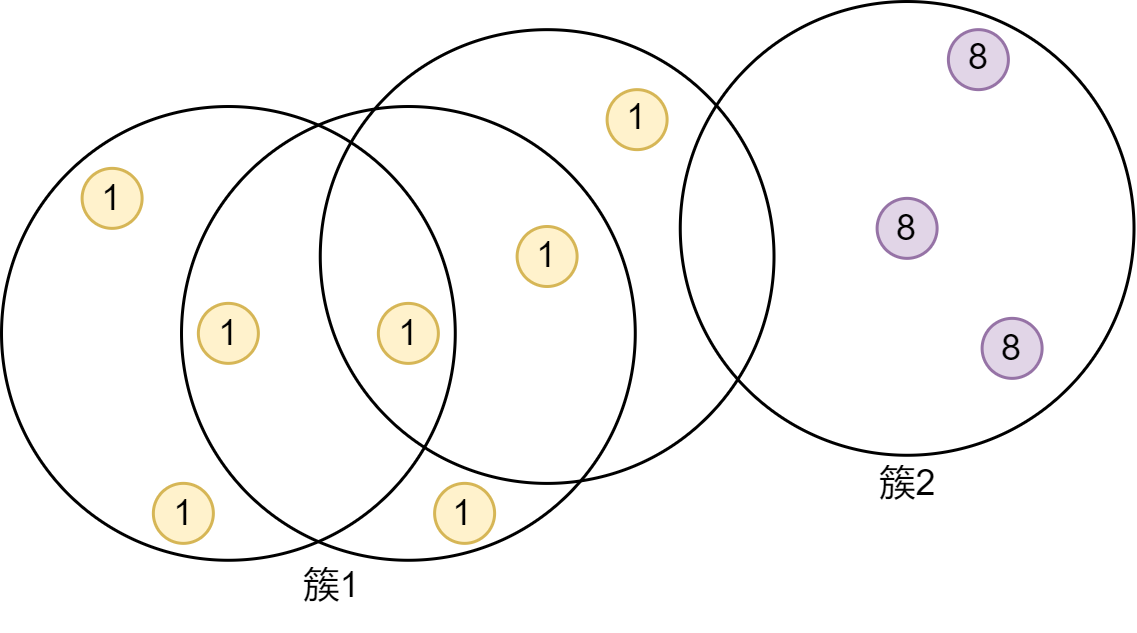
\includegraphics[width=0.5\textwidth]{../img/dbres.png}
	\caption{还原聚类结果}
	\label{dbres}
\end{figure}

\begin{algorithm}[htbp]
	\renewcommand{\algorithmicrequire}{\textbf{输入:}}
	\renewcommand{\algorithmicensure}{\textbf{输出:}}
	\caption{密度聚类}
	\label{alg_t1_s2}
	\begin{algorithmic}[1]
		\REQUIRE 数组sharedList简写为d,相邻关系$ u_{ij},i,j\in[n] $
		\ENSURE 簇连接关系$ plist $
		\FOR{$ i=1 $ to $ n $}
		\FOR {$ j=1 $ to $ n $}
		\STATE $ m_1 \leftarrow \text{MUL}(d[i].isCore, u_{ij}, 1-d[j].isCore) $
		\STATE $ m_2 \leftarrow \text{MUL}(m_1, 1-d[j].isMark) $
		\STATE $ d[j].cluId \leftarrow  \text{MUL}(m_2, d[i].cluId) + \text{MUL}(1-m_2, d[j].cluId)$
		\STATE $ conn \leftarrow \text{MUL}(d[i].isCore, d[j].isCore, u_{ij}) $
		\STATE add new info item $ [d[i].cluId, d[j].cluId, conn] $ to plist
		\STATE $ d[j].isMark \leftarrow m_1 + d[j].isMark - \text{MUL}(m_1, d[j].isMark) $
		\ENDFOR
		\ENDFOR
	\end{algorithmic}
\end{algorithm}

\begin{tabular}{c|l}
	$ x_i =\{x_{i1},...,x_{im}\} $ & 维度为$ m $的数据点$ x_i $\\
	$ C = \{c_1,...,c_m\} $& Kd-tree中每个点的中心\\
	$ Z = \{z_1,...,z_k\} $& $ k $个候选簇\\
	$ \langle x \rangle/\langle x \rangle^A $& $ x $在$ \mathbb{Z}_n $上的加性秘密共享值\\
	$ \langle x \rangle^B $& $ x $在$ \mathbb{Z}_2 $上的布尔共享值\\
	MUL & 安全乘法\\
	SED & 带缩放因子的安全欧式距离计算协议\\
	SC & 安全比较协议\\
	SMin(S/L) & 安全极值计算协议(大数据集/小数据集)\\
	SF & 安全过滤协议\\
	SSORT & 安全排序协议\\
	DIST & 安全欧式距离计算\\
	
\end{tabular}

\end{document}
